\documentclass[handout]{beamer}
\setbeamertemplate{footline}[frame number]

\ifx\pdfoutput\undefined
%  \usepackage{graphicx}
\else
%  \usepackage[pdftex]{graphicx}
  \DeclareGraphicsRule{*}{mps}{*}{}
\fi

%%\documentclass[landscape]{slides}
%\AtBeginDocument{%
%  \pdfpageheight = \paperheight
%  \pdfpagewidth = \paperwidth
%}

%%\usepackage{times}
\usepackage{color}
\usepackage{latexsym}
%\usepackage{graphicx}

\raggedright

\definecolor{bgblue}{rgb}{0.04,0.39,0.53}

\newcommand{\argmax}[1]{\begin{array}{c}\mbox{arg max}\\#1\end{array}}

\begin{document}


\title{\color{blue}Natural Language Processing}

\author{Anoop Sarkar \\ {\tt http://anoopsarkar.github.io/nlp-class}}
\institute{}
%\date{}
     
{
\setbeamertemplate{navigation symbols}{}
\addtocounter{framenumber}{-1}
\begin{frame}
\begin{center}
\vspace{1cm}

\includegraphics[scale=0.4]{figures/natlang-cky-logo.eps}
\end{center}
\titlepage
\end{frame}
}



%\section*{Outline}
%\frame{
%\frametitle{Outline}
%\tableofcontents
%}

\section{Quick Guide to Probability Theory}
\frame{\tableofcontents[currentsection]}

\begin{frame}
\frametitle{Quick guide to probability theory}
\begin{itemize}[<+->]
\item P(X) means probability that X is true
\begin{itemize}[<+->]
\item P(baby is a girl) $= 0.5$ \\
percentage of total number of babies that are girls
\item P(baby girl is named Kiki) $= 0.001$ \\
percentage of total number of babies that are named Kiki
\end{itemize}
\end{itemize}
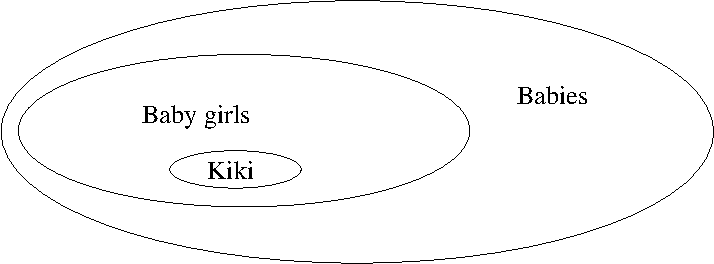
\includegraphics[scale=.8]{figures/prob-fig1}
\end{frame}

%\begin{frame}
%\frametitle{Probability: What does it really
%  mean?}
%\begin{itemize}[<+->]
%\item P(GC drinks and drives $\mid$ GC is in Hawaii) $= 0.9$

%\begin{itemize}[<+->]
%\item GC drove drunk 90\% of the time when in Hawaii -- {\color{blue} Frequentist}
%\item If GC visited Hawaii infinitely many times $\ldots$ -- {\color{blue} Estimation}
%\item I would bet at 90 to 1 odds that GC drinks and drives when in Hawaii (degree of belief) -- {\color{blue} Bayesian}
%\end{itemize}
%\end{itemize}
%\end{frame}

\begin{frame}
\frametitle{Joint probability}
\begin{itemize}[<+->]
\item P(X,Y) means probability that X and Y are both true
\begin{itemize}[<+->]
\item P(baby girl, blue eyes)
percentage of total number of babies that are girls and have blue eyes
\end{itemize}
\end{itemize}
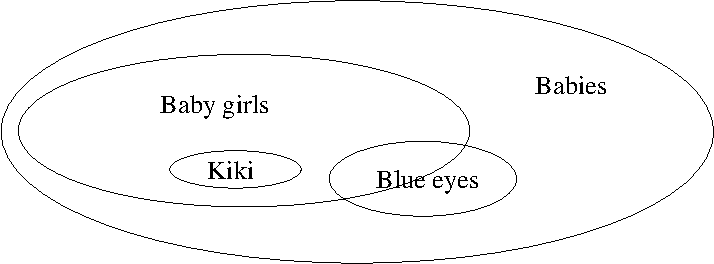
\includegraphics[scale=.8]{figures/prob-fig2}

\end{frame}

\begin{frame}
\frametitle{Conditional probability}
\begin{itemize}[<+->]
\item P(X $\mid$ Y) means probability that X is true when we already know
  that Y is true
\begin{itemize}[<+->]
\item P(baby is named Kiki $\mid$ baby is a girl) $= 0.002$
\item P(baby is a girl $\mid$ baby is named Kiki) $= 1$
\end{itemize}
\end{itemize}
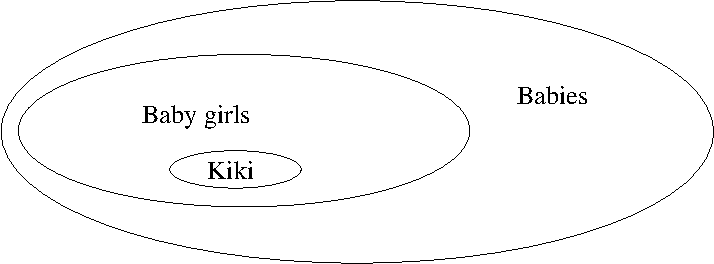
\includegraphics[scale=.8]{figures/prob-fig1}

\end{frame}

\begin{frame}
\frametitle{Conditional probability}
\begin{itemize}[<+->]
\item Conditional and joint probabilities are related:
\[ P(X \mid Y) = \frac{P(X,Y)}{P(Y)} \]

\begin{itemize}[<+->]
\item $P(\mbox{baby is named Kiki} \mid \mbox{baby is a girl}) =
  \frac{P(\mbox{baby is a girl}, \mbox{baby is named Kiki})}{P(\mbox{baby is
    a girl})} = \frac{0.001}{0.5} = 0.002 $
\end{itemize}
\end{itemize}
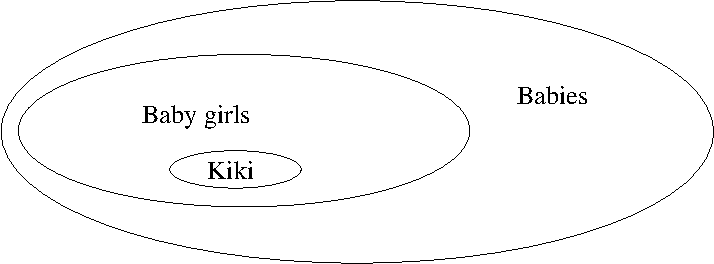
\includegraphics[scale=.8]{figures/prob-fig1}

\end{frame}

\begin{frame}
\frametitle{Bayes rule}
\begin{itemize}[<+->]
\item Conditional probability re-written as likelihood times prior:
\[ P(X \mid Y) = \frac{P(Y \mid X) \times P(X)}{P(Y)} \]

\begin{itemize}[<+->]
\item $P(\mbox{named Kiki} \mid \mbox{girl}) =
  \frac{P(\mbox{girl} \mid \mbox{named Kiki}) \times P(\mbox{named
  Kiki})}{P(\mbox{girl})} = \frac{1.0 \times 0.001}{0.5} = 0.002$
\end{itemize}
\end{itemize}
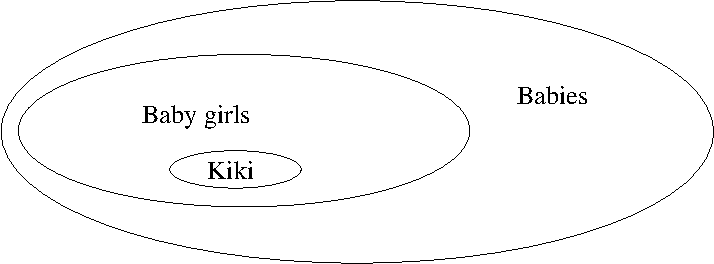
\includegraphics[scale=.8]{figures/prob-fig1}

\end{frame}

\begin{frame}
\frametitle{Bayes Rule}
\begin{center}
\begin{eqnarray}
P(X \mid Y) &= &\frac{P(X,Y)}{P(Y)} \\
P(Y \mid X) &= &\frac{P(Y,X)}{P(X)} \\
P(X,Y) &= &P(Y,X) \\
P(X \mid Y) \times P(Y) &= &P(Y \mid X) \times P(X) \\
P(X \mid Y) &= &\frac{P(Y \mid X) \times P(X)}{P(Y)} \\
P(X \mid Y) &= &P(Y \mid X) \times P(X)
\end{eqnarray}
\end{center}   

\end{frame}

\begin{frame}
\frametitle{Basic Terms}
\begin{itemize}[<+->]
\item $P(e)$ -- {\em a priori} probability or just {\em prior}
\item $P(f \mid e)$ -- {\em conditional} probability. The chance of
  $f$ given $e$
\item $P(e, f)$ -- {\em joint} probability. The chance of $e$ and $f$
  both happening.
\item If $e$ and $f$ are {\em independent} then we can write $P(e,f) =
  P(e) \times P(f)$
\item If $e$ and $f$ are not {\em independent} then we can write
  $P(e,f) = P(e) \times P(f \mid e)$ \\
 $P(e,f) = P(f) \times\ ?$
\end{itemize}

\end{frame}

\begin{frame}
\frametitle{Basic Terms}
\begin{itemize}[<+->]
\item Addition of integers: \[ \sum_{i=1}^n i = 1 + 2 + 3 + \ldots +
  n \]
\item Product of integers: \[ \prod_{i=1}^n i = 1 \times 2 \times 3
  \times \ldots \times n \]
\item Factoring: \[ \sum_{i=1}^n i \times k = k + 2k + 3k + \ldots + nk
  = k \sum_{i=1}^n i \]
\item Product with constant: \[ \prod_{i=1}^n i \times k = \pause 1 k \times 2 k \ldots \times n k = \pause k^n \times \prod_{i=1}^n i \]
\end{itemize}

\end{frame}

\begin{frame}
\frametitle{Probability: Axioms}
\begin{itemize}[<+->]
\item $P$ measures total probability of a set of events
\item $P(\emptyset) = 0$
\item $P(\mbox{all events}) = 1$
\item $P(X) \leq P(Y)$ for any $X \subseteq Y$
\item $P(X) + P(Y) = P(X \cup Y)$ provided that $X \cap Y = \emptyset$
\begin{itemize}
\item $P$(Kiki is a girl) + $P$(Kiki is fictional) = \\
$P$(Kiki is a fictional girl), \\
provided there are no real girls called Kiki or persons/objects that are fictional Kiki's.
\end{itemize}

\end{itemize}

\end{frame}

\begin{frame}
\frametitle{Probability Axioms}
\begin{itemize}[<+->]
\item All events sum to 1: \[ \sum_e P(e) = 1 \]
\item Marginal probability $P(f)$: \[ P(f) = \sum_e P(e, f)  \]
\item Conditional probability: \[ \sum_e P(e \mid f) = \pause \sum_e \frac{P(e,f)}{P(f)} = \pause \frac{1}{P(f)} \sum_e P(e,f) = \pause 1 \]
\item Computing $P(f)$ from axioms: \[ P(f) = \sum_e P(e) \times
  P(f \mid e) \]
\end{itemize}

\end{frame}

\begin{frame}
\frametitle{Probability: The Chain Rule}
\begin{itemize}[<+->]
\item $P(a,b,c,d \mid e)$
\item We cannot simply remove items from the left of $\mid$ \\
(verify that it violates the definitions we have given based on sets)
\item In this case we can use the chain rule of probability to rescue
  us
\item $P(a,b,c,d \mid e) = $\\
$P(d \mid e) \cdot P(c \mid d,e) \cdot P(b \mid c,d,e) \cdot P(a \mid b,c,d,e)$ 
\item To see why this is possible, recall that \( P(X \mid Y) = \frac{p(X,Y)}{p(Y)} \)
\begin{itemize}
\item $\frac{ p(a,b,c,d,e) }{ p(e) } = \frac{p(d,e)}{p(e)} \cdot \frac{p(c,d,e)}{p(d,e)} \cdot \frac{p(b,c,d,e)}{p(c,d,e)} \cdot \frac{p(a,b,c,d,e)}{p(b,c,d,e)} $
\end{itemize}
\item Use chain rule and simplify:
\[ P(a,b,c,d \mid e) = P(d \mid e) \cdot P(c \mid d, e) \cdot P(b \mid c, e) \cdot P(a \mid b, e) \]
\end{itemize}

\end{frame}

\begin{frame}
\frametitle{Probability: The Chain Rule}
\begin{itemize}[<+->]
\item $P(e_1, e_2, \ldots, e_n) = P(e_1) \times P(e_2 \mid
  e_1) \times P(e_3 \mid e_1, e_2) \ldots $ 
\[ P(e_1, e_2, \ldots, e_n) = \prod^n_{i=1} P(e_i \mid e_{i-1},
  e_{i-2}, \ldots, e_1) \]
\end{itemize}

\end{frame}

\begin{frame}
\frametitle{Probability: Random Variables and Events}
\begin{itemize}[<+->]
\item What is $y$ in $P(y)$ ?
\item Shorthand for value assigned to a random variable $Y$, e.g. $Y = y$
\item $y$ is an element of some implicit {\bf event space}: ${\cal E}$
\end{itemize}

\end{frame}

\begin{frame}
\frametitle{Probability: Random Variables and Events}
\begin{itemize}[<+->]
\item The {\em marginal probability} $P(y)$ can be computed from $P(x,y)$ as
  follows:
\[ P(y) = \sum_{x \in {\cal E}} P(x,y) \]
\item Finding the value that maximizes the probability value:
\[ \hat{x} = \argmax{x \in {\cal E}} P(x) \]
\end{itemize}

\end{frame}

\section{Log Probability}
\frame{\tableofcontents[currentsection]}

\begin{frame}
\frametitle{Log Probability Arithmetic}
\begin{itemize}[<+->]
\item Practical problem with tiny $P(e)$ numbers: underflow
\item One solution is to use log probabilities:
\begin{eqnarray}
\log(P(e)) &=& \log(p_1 \times p_2 \times \ldots \times p_n) \nonumber
\\
&=& \log(p_1) + \log(p_2) + \ldots + \log(p_n) \nonumber
\end{eqnarray}
\item Note that: \[ x = \exp(\log(x)) \]
\item Also more efficient: addition instead of multiplication
\end{itemize}

\end{frame}

\begin{frame}
\frametitle{Log Probability Arithmetic}
\begin{center}
\begin{tabular}{|c|c|}
\hline
$p$ & $\log(p)$ \\
\hline
$0.0$ & $- \infty$ \\
$0.1$ & $-3.32$ \\
$0.2$ & $-2.32$ \\
$0.3$ & $-1.74$ \\
$0.4$ & $-1.32$ \\
$0.5$ & $-1.00$ \\
$0.6$ & $-0.74$ \\
$0.7$ & $-0.51$ \\
$0.8$ & $-0.32$ \\
$0.9$ & $-0.15$ \\
$1.0$ & $0.00$ \\
\hline
\end{tabular}
\end{center}

\end{frame}

\begin{frame}
\frametitle{Log Probability Arithmetic}
\begin{itemize}[<+->]
\item So: $(0.5 \times 0.5 \times \ldots 0.5) = (0.5)^n$ might get too
  small but $(- 1 - 1 - 1 - 1) = - n$ is manageable
\item Another useful fact when writing code \\
($\log_2$ is {\em log to the base 2}):
\[ \log_2(x) = \frac{\log_{10}(x)}{\log_{10}(2)} \]
\end{itemize}

\end{frame}

\begin{frame}
\frametitle{Log Probability Arithmetic}
\begin{itemize}[<+->]
\item Adding probabilities is expensive to compute: $logadd(x,y) = \log(\exp(x) + \exp(y))$
\item A more efficient soln, let $big$ be a large constant e.g. $10^{30}$:
\begin{tabbing}
\=123\=568\=901\=23\=\kill \\
\textsf{function } $logadd(x,y):$ {\color{red} \# returns $\log(\exp(x) + \exp(y))$} \\
\>  \textsf{if } $(y - x) > \log(big)$ \color{blue} \textsf{return } $y$ \\
\>  \textsf{elsif  } $(x - y) > \log(big)$ \color{blue} \textsf{return } $x$ \\
\>  \textsf{else } \color{blue} \textsf{return } \\
\>\>\> \color{blue} $min(x, y) + \log(\exp(x - min(x,y)) + \exp(y -
min(x,y)))$ \\
\>  \textsf{endif }
\end{tabbing}
\item There is a more efficient way of computing $\log(\exp(x - 
min(x,y)) + \exp(y - min(x,y)))$
\end{itemize}

\end{frame}

\begin{frame}
\frametitle{Log Probability Arithmetic}
\begin{center}
\begin{tabbing}
123\=123\=568\=901\=23\=\kill \\
\textsf{function } $logadd(x,y):$ \\
\>  \textsf{if } $(y - x) > \log(big)$ \textsf{return } $y$ \\
\>  \textsf{elsif  } $(x - y) > \log(big)$ \textsf{return } $x$ \\
\>  \textsf{elsif ($x \geq y$)} \color{blue} return $x + \log(1 + \exp(y-x))$ \\
\>\> \color{red} \# {\small note that $max(x,y) = x$ and $y-x \leq 0$} \\
\> else \color{blue} return $y + \log(\exp(x-y) + 1)$ \\
\>\> \color{red} \# {\small note that $max(x,y) = y$ and $x-y \leq 0$} \\
\>  \textsf{endif } \\
\color{red} {\small Also, in ANSI C, {\tt log1p} efficiently computes $\log(1+x)$} \\
\color{red} {\footnotesize\tt http://www.ling.ohio-state.edu/\~{}jansche/src/logadd.c} \\
{\small In Python, numpy.logaddexp2(x1,x2) for base 2} 
\end{tabbing}
\end{center}

\end{frame}

\section{Basics of Information Theory}
\frame{\tableofcontents[currentsection]}

\begin{frame}
\frametitle{Information Theory}
\begin{itemize}[<+->]
\item Information theory is the use of probability theory to quantify
  and measure ``information''.
\item Consider the task of efficiently sending a message. Sender Alice
  wants to send several messages to Receiver Bob. Alice wants to do
  this as efficiently as possible.
\item Let's say that Alice is sending a message where the entire
  message is just one character {\em a}, e.g. {\em aaaa$\ldots$}. In
  this case we can save space by simply sending the length of the
  message and the single character.
\end{itemize}

\end{frame}

\begin{frame}
\frametitle{Information Theory}
\begin{itemize}[<+->]
\item Now let's say that Alice is sending a completely random signal to
  Bob. If it is random then we cannot exploit anything in the message
  to compress it any further.
\item The {\em expected} number of bits it takes to transmit
  some infinite set of messages is what is called entropy. 
\item This formulation of entropy by Claude Shannon was adapted from
  thermodynamics, converting information into a quantity that can be measured.
\item Information theory is built around this notion of message
  compression as a way to evaluate the amount of information. 
\end{itemize}

\end{frame}

\begin{frame}[fragile]
\frametitle{Expectation}
\begin{itemize}[<+->]
\item For a probability distribution $p$
\item \textbf{Expectation} with respect to $p$ is a weighted average:
\begin{eqnarray*}
 E_p[x] &=& \frac{x_1 \cdot p_1 + x_2 \cdot p_2 + \ldots + x_n p_n}{p_1 + p_2 + \ldots + p_n} \\
  &=& x_1 \cdot p_1 + x_2 \cdot p_2 + \ldots + x_n p_n \\
  &=& \sum_{x \in {\cal E}} x \cdot p(x) 
\end{eqnarray*}
\item Example: for a six-sided die the expectation is:
\[ E_p[x] = 1 \cdot \frac{1}{6} + 2 \cdot \frac{1}{6} + \ldots + 6 \cdot \frac{1}{6} = 3.5 \]
\end{itemize}

\end{frame}

\begin{frame}
\frametitle{Entropy}
\begin{itemize}[<+->]
\item For a probability distribution $p$
\item \textbf{Entropy} of $p$ is: 
\[ H(p) = - \sum_{x \in {\cal E}} p(x) \cdot \log_2 p(x) \]
\item Any base can be used for the $\log$, but base $2$ means
  that entropy is measured in bits.
\item What is the {\it expected} number of bits with respect to $p$:
\[ - E_p [ \log_2 p(x) ] = H(p) \]
\item Entropy answers the question: {\it What is the expected
  number of bits needed to transmit messages from event 
  space ${\cal E}$, where $p(x)$ defines the probability of observing $x$?} 
\end{itemize}

\end{frame}

\begin{frame}
\frametitle{Entropy}
\begin{itemize}[<+->]
\item Alice wants to bet on a horse race. She has to send a message to
  her bookie Bob to tell him which horse to bet on.
\item There are 8 horses. One encoding scheme for the messages is to
  use a number for each horse. So in bits this would be $001, 010,
  \ldots$\\
(lower bound on message length = 3 bits in this encoding scheme) 
\item Can we do better?
\end{itemize}

\end{frame}

\begin{frame}
\frametitle{Entropy}
\begin{center}
\begin{tabular}{|cc|cc|}
\hline
Horse 1 & $\frac{1}{2}$ & Horse 5 & $\frac{1}{64}$ \\
\hline
Horse 2 & $\frac{1}{4}$ & Horse 6 & $\frac{1}{64}$ \\
\hline
Horse 3 & $\frac{1}{8}$ & Horse 7 & $\frac{1}{64}$ \\
\hline
Horse 4 & $\frac{1}{16}$ & Horse 8 & $\frac{1}{64}$ \\
\hline
\end{tabular}
\end{center}
\begin{itemize}[<+->]
\item If we know how likely we are to bet on each horse, say based on
  the horse's probability of winning, then we can do better.
\item Let $p$ be the probability distribution given in the
table above. The entropy of $p$ is $H(p)$
\end{itemize}

\end{frame}

\begin{frame}
\frametitle{Entropy}
\begin{eqnarray*}
\lefteqn{ H(p) = } \nonumber \\
&=& - \sum^{8}_{i=1} p(i) \log_2\ p(i) \nonumber \\
&=& - \left( \frac{1}{2} \log_2 \frac{1}{2} + \frac{1}{4} \log_2 \frac{1}{4} +
\frac{1}{8} \log_2 \frac{1}{8} + \frac{1}{16} \log_2 \frac{1}{16} +
4 (\frac{1}{64} \log_2 \frac{1}{64}) \right) \nonumber \\
&=& - \left( \frac{1}{2} \times -1 + \frac{1}{4} \times -2 +
\frac{1}{8} \times -3 + \frac{1}{16} \times -4 +
4 (\frac{1}{64} \times -6 ) \right) \nonumber \\
&=& - \left( {\color{red}-\frac{1}{2} - \frac{1}{2}} {\color{blue} - \frac{3}{8} - \frac{1}{4} - \frac{3}{8}} \right) \nonumber \\
&=& 2\ \textit{bits}
\end{eqnarray*}

\begin{itemize}[<+->]
\item What is the entropy when the horses are equally likely to win?
\[ H(\textit{uniform distribution}) = - 8 (\frac{1}{8} \times -3) = 3 \textit{ bits} \]
\end{itemize}

\end{frame}

\begin{frame}
\frametitle{Entropy}
\begin{itemize}[<+->]
\item e.g., most likely horse gets code $0$, next most likely gets $10$, and then $110, 1110, \ldots$ \\ {\small many possible coding schemes, this is a simple code to illustrate number of bits needed for a large number of messages \ldots}
\item Assume there are $320$ messages (one for each race): \\
code $0$ occurs 160 times, code $10$ occurs 80 times, code $110$ occurs 40 times, code $1110$ occurs 20 times, code $11110$ occurs 5 times.
\item Total number of bits for all messages: 160*len(0) + 80*len(10) + 40*len(110) + 20*len(1110) + 5*len(11110) 
\item Number of bits: 160*1 + 80*2 + 40*3 + 20*4 + 5*5 = 545
\item Total number of bits per message (per race): $\frac{545}{320} \approx$ 1.7 bits (always less than 2 bits)
\end{itemize}

\end{frame}

\begin{frame}
\frametitle{Perplexity}
\begin{itemize}[<+->]
\item The value $2^{H(p)}$ is called the {\bf perplexity} of a distribution $p$
\item Perplexity is the weighted average number of choices a random
  variable has to make.
\item Choosing between 8 equally likely horses (H=3) is $2^3 = 8$.
\item Choosing between the biased horses from before (H=2) is $2^2 =
  4$. 
\end{itemize}

\end{frame}

\begin{frame}
\frametitle{Relative Entropy}
\begin{itemize}[<+->]
\item In real life, we cannot know for sure the exact winning
  probability for each horse. 
\item Let's say $q$ is the estimate
  and $p$ is the true probability \\
  {\small (say we got $q$ by observing previous races with these horses)}
\item We define the {\em distance} between $q$ and $p$ as the {\bf relative entropy}: written as $D(q \| p)$
\[ D(q \| p) = - \sum_{x \in {\cal E}} q(x) \log_2 \frac{p(x)}{q(x)} \]
\item Note that
\[ D(q \| p) = - E_{ q(x) } \left[ \log_2 \frac{p(x)}{q(x)} \right] \]
\item The relative entropy is also called the {\em Kullback-Leibler divergence}.
\end{itemize}

\end{frame}

\begin{frame}
\frametitle{Cross Entropy and Relative Entropy}
\begin{itemize}[<+->]
\item The {\bf relative entropy} can be written as the sum of two terms:
\begin{eqnarray*}
D(q \| p) & = & - \sum_{x \in {\cal E}} q(x) \log_2 \frac{p(x)}{q(x)} \\
& = & - \sum_{x} q(x) \log_2 p(x) + \sum_{x} q(x) \log_2 q(x) 
\end{eqnarray*}
\item We know that $H(q) = - \sum_{x} q(x) \log_2 q(x)$
\item Similarly define $H_{q}(p) = - \sum_{x} q(x) \log_2 p(x)$
\[
\begin{array}{l@{}c@{}l@{}c@{}l@{}}
D(q \| p) & = & H_{q}(p) & - & H(q) \\
\textbf{relative entropy}(q, p) & = & \textbf{cross entropy}(q, p) & - & \textbf{entropy}(q) 
\end{array}
\]
\item The term $H_{q}(p)$ is called the {\bf cross entropy}.
\end{itemize}

\end{frame}

\begin{frame}
\frametitle{Cross Entropy and Relative Entropy}
\begin{itemize}[<+->]
\item $H_{q}(p) \geq H(q)$ always.
\item $D(q \| p) \geq 0$ always, and $D(q \| p) = 0$ iff $q = p$
\item $D(q \| p)$ is not a true distance: 
  \begin{itemize}
  \item It is asymmetric: $D(q \| p) \neq D(p \| q)$, 
  \item It does not obey the triangle inequality: $D(p \| r) \nleq D(p \| q) + D(q \| r)$
  \end{itemize}
%\item Pinsker's inequality (sup is the lowest upper bound): 
%\[ \sqrt{ \frac{ D(q \| p) }{ 2 } } \geq \sup \{ | q(x) - p(x) | \} \]
\end{itemize}

\end{frame}

\begin{frame}
\frametitle{Conditional Entropy and Mutual Information}
\begin{itemize}[<+->]
\item {\it Entropy} of a random variable $X$:
\[ H(X) = - \sum_{x \in {\cal E}} p(x) \log_2 p(x) \]
\item {\it Conditional Entropy} between two random variables $X$ and $Y$:
\[ H(X \mid Y) = - \sum_{x,y \in {\cal E}} p(x,y) \log_2 p(x
\mid y) \]
\item {\it Mutual Information} between two random variables $X$ and $Y$:
\[ I(X;Y) = D(p(x,y) \| p(x)p(y)) = \sum_x \sum_y p(x,y) \log_2
\frac{p(x,y)}{p(x)p(y)} \]
\end{itemize}

\end{frame}

\end{document}

